\section{Resultados del Algoritmo Genético}

En esta sección presentamos los resultados obtenidos con el AG. Para obtener la matriz con la asignación final se simularon $6$ generaciones (población inicial más 5 reemplazamientos). El tamaño de la población para cada generación es $10$. El número de genes varía dependiendo de cada asignación.


En la \figurename{~\ref{EjcalifMejoresHijos}} vemos las calificaciones de la mejor asignación por generación. Observamos que la mejora en la calificación es considerable de la población inicial a la segunda generación. Notamos que la calificación del mejor elemento de la generación 5 fue menor al de la generación 4.

\begin{figure}[H]
\centering
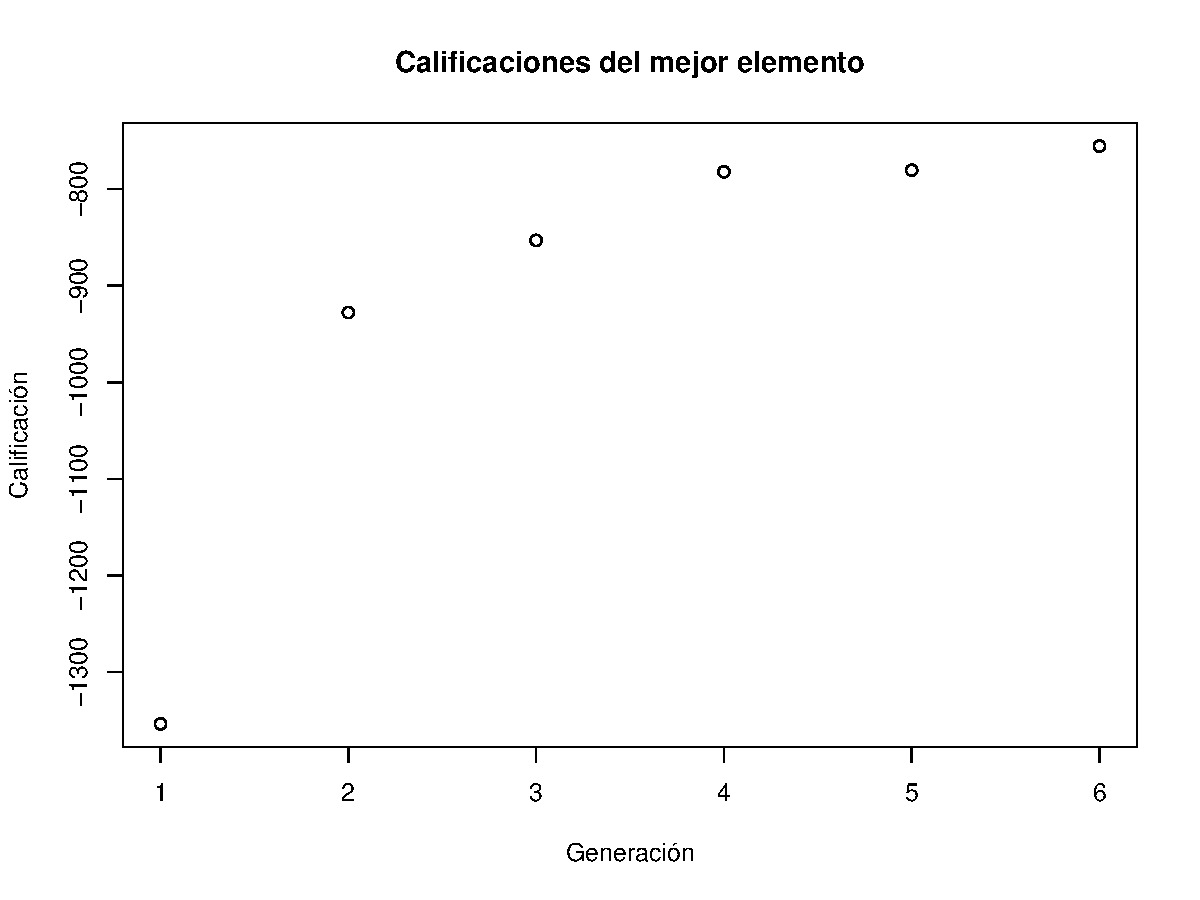
\includegraphics[width=\textwidth]{calif_mejores_hijos.pdf} %scale = 0.7
\caption[\textit{Calificaciones de mejores asignaciones}]{\textit{Se muestran las calificaciones de la mejor asignación por generación. Se observa una mejora considerable en la calificación de la generación 1 a la 2.}}\label{EjcalifMejoresHijos}
\end{figure}

%En la \figurename{~\ref{EjcalifAsig}} vemos las calificaciones de las asignaciones.
%
%\begin{figure}[H]
%\centering
%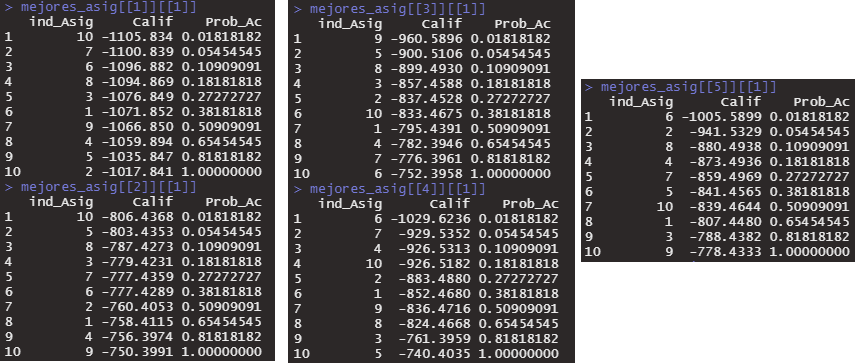
\includegraphics[width=\textwidth]{ej_calif_asignaciones} %scale = 0.7
%\caption{\textit{Ejemplo con calificaciones de asignaciones.}}\label{EjcalifAsig}
%\end{figure}

%En la \figurename{~\ref{EjcalifAsig_x_generacion}} vemos las calificaciones de las asignaciones por generación. Cada línea representa una generación. De abajo hacia arriba se tiene de la primer población a la sexta. Podemos ver que las calificaciones de las poblaciones 4 y 5 son muy parecidas. Al igual que en la \figurename{~\ref{EjcalifMejoresHijos}}, se puede observar una mejora considerable en las calificaciones de las asignaciones de la generación 1 a la 2.
%
%\begin{figure}[H]
%\centering
%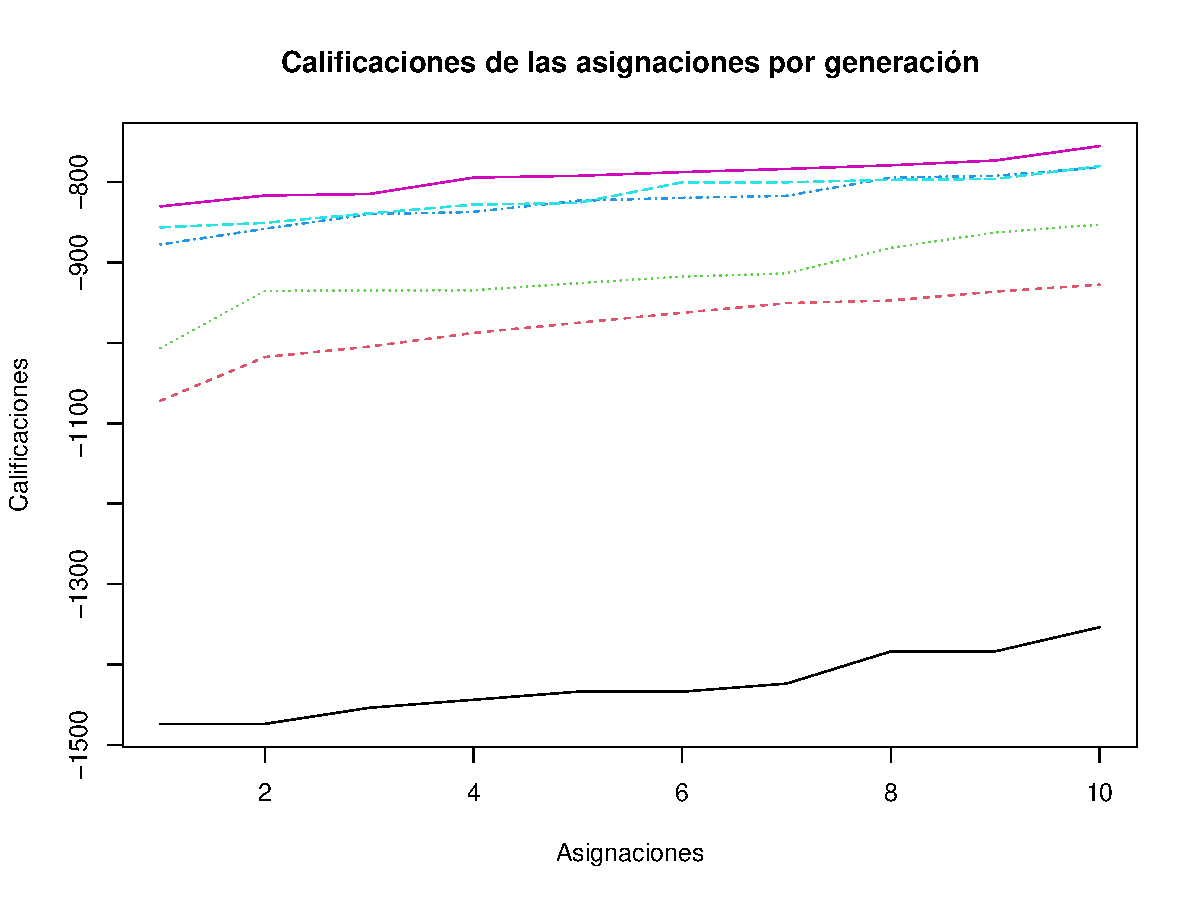
\includegraphics[width=\textwidth]{calif_asig_x_generacion.pdf} %scale = 0.7
%\caption[\textit{Calificaciones de asignaciones por generación}]{\textit{Se muestran las calificaciones de las asignaciones por generación. Se observa una mejora considerable en la calificación de la generación 1 a la 2.}}\label{EjcalifAsig_x_generacion}
%\end{figure}


\begin{figure}[H]
\centering
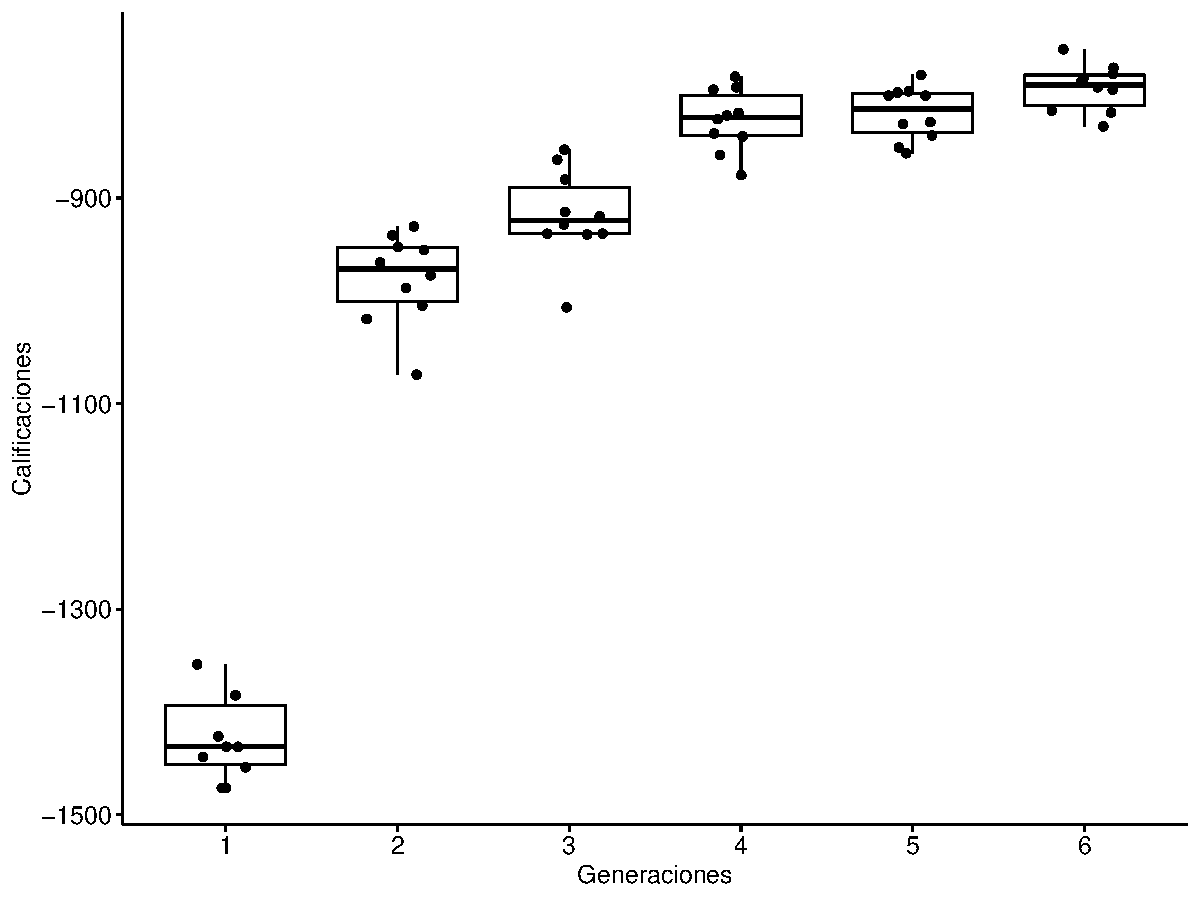
\includegraphics[width=\textwidth]{boxplot_calif_x_generacion.pdf} %scale = 0.7
\caption[\textit{Gráfica de caja de calificaciones de asignaciones por generación}]{\textit{Se muestra la gráfica de caja de las calificaciones de las asignaciones por generación. Se observa una mejora considerable en la calificación de la generación 1 a la 2. Los puntos respresentan las calificaciones de cada asignación por generación.}}\label{boxplot_calif_x_generacion}
\end{figure}

\begin{figure}[H]
\centering
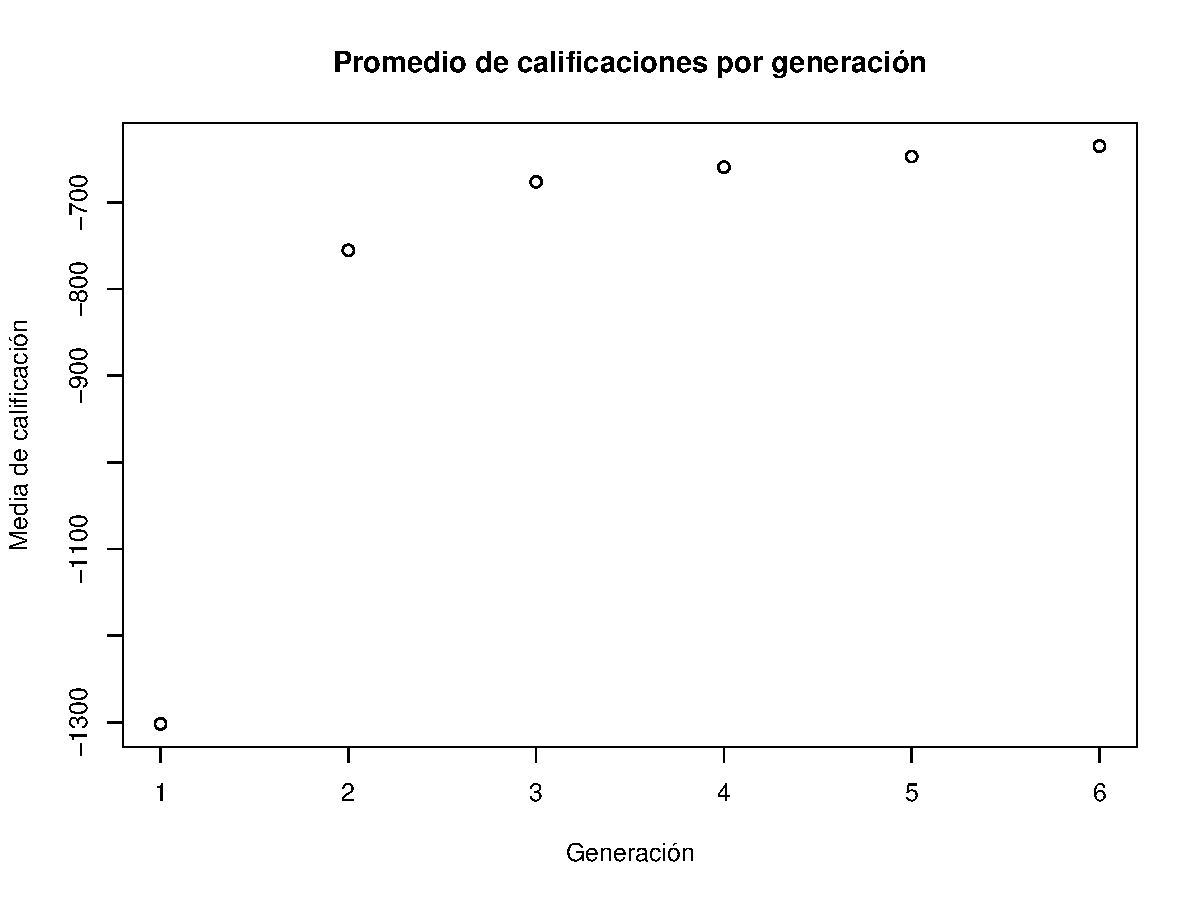
\includegraphics[width=\textwidth]{media_calif_x_generacion.pdf} %scale = 0.7
\caption[\textit{Media de calificaciones de asignaciones por generación}]{\textit{Se muestra el promedio de las calificaciones de las asignaciones por generación. Se observa una mejora considerable en la calificación de la generación 1 a la 2.}}\label{media_calif_x_generacion}
\end{figure}


\begin{figure}[H]
\centering
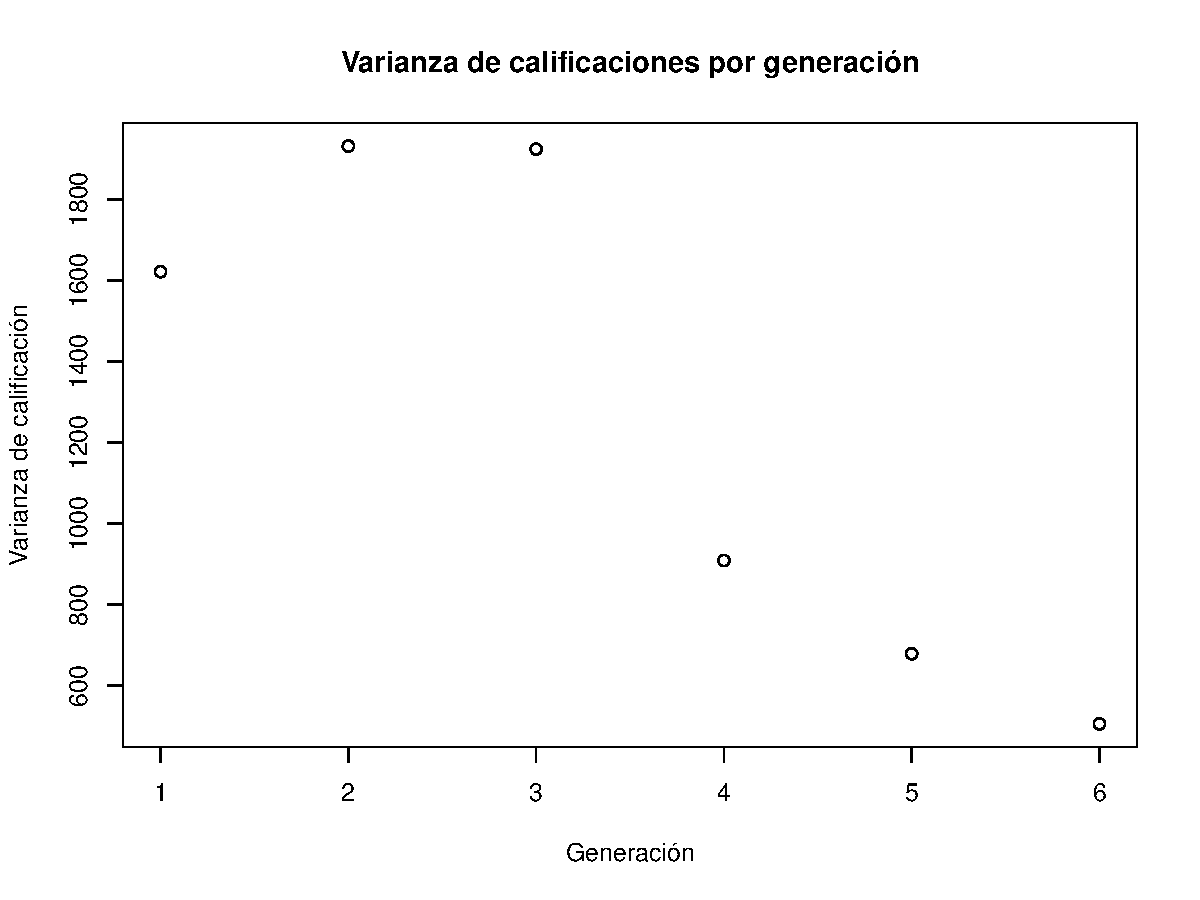
\includegraphics[width=\textwidth]{varianza_calif_x_generacion.pdf} %scale = 0.7
\caption[\textit{Varianza de calificaciones de asignaciones por generación}]{\textit{Se muestra la varianza de las calificaciones de las asignaciones por generación. Se observa una disminución considerable de la generación 3 a la 4.}}\label{var_calif_x_generacion}
\end{figure}


\begin{figure}[H]
\centering
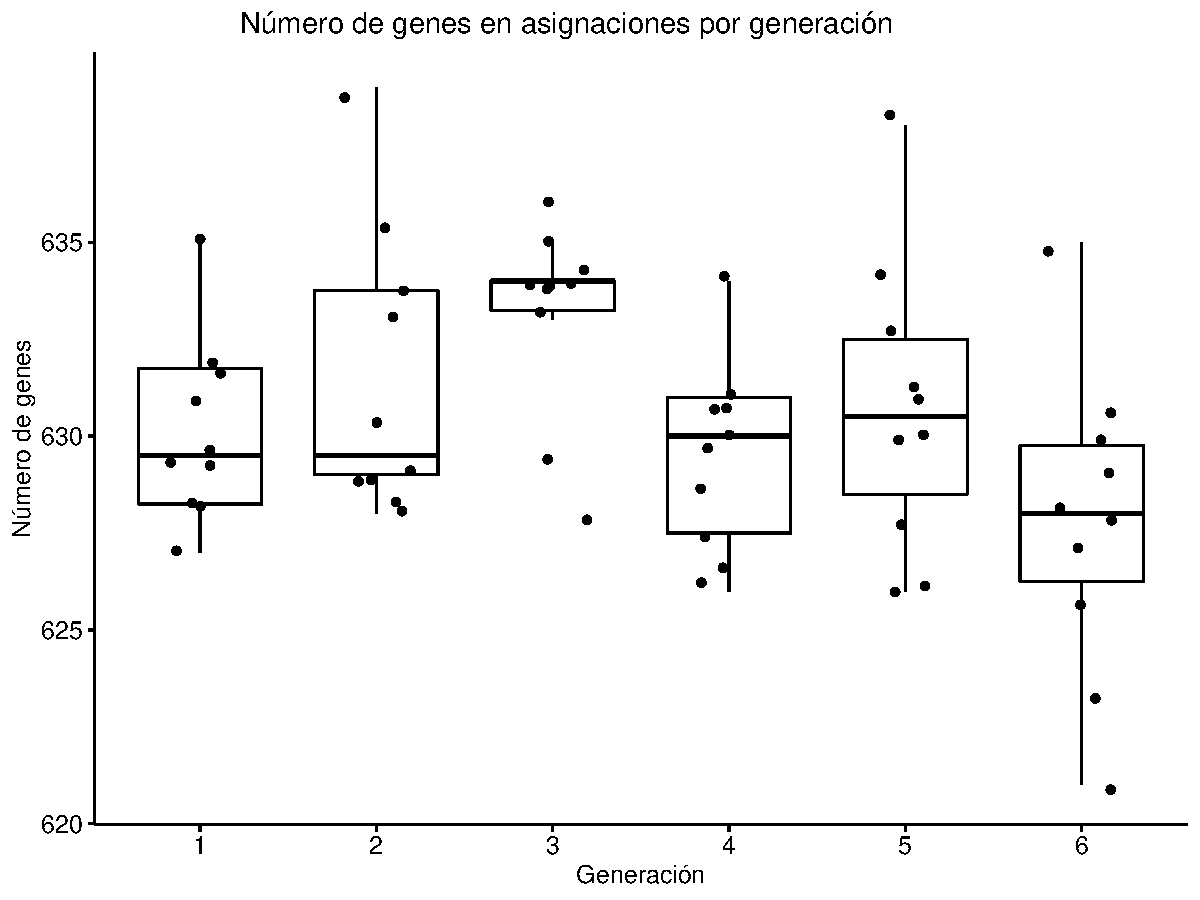
\includegraphics[width=\textwidth]{boxplot_num_genes_x_generacion.pdf} %scale = 0.7
\caption[\textit{Gráfica de caja del número de genes en asignaciones por generación}]{\textit{Se muestra la gráfica de caja del número de genes en asignaciones por generación. Se observa que los valores permanecen constantes. Los puntos respresentan el número de genes de cada asignación por generación.}}\label{boxplot_num_genes_x_generacion}
\end{figure}


%En un esqueleto simulado para el 2020-2 se tuvieron 1018 grupos. De éstos se asignaron 612. Encontramos que 262 grupos sin asignación correspondían a materias optativas. Prácticamente $\dfrac{1}{4}$ de los grupos no asignados son de materias optativas. Ésto se debe a que se pueden asignar \textit{num\_max\_asig} materias obligatorias a los profesores por lo que ya no se les asignan las optativas. En la matriz de solicitudes puede haber grupos que no están en la asignación final. Ésto por el cruce de los padres.
%
%\begin{eqnarray*}
%\dfrac{612}{1018} &=& 60.11\% \text{grupos asignados}\\
%\dfrac{262}{1018} &=& 25.73\% \text{grupos de optativas sin asignación}\\
%\dfrac{1018 - (612 + 262)}{1018} &=& \dfrac{144}{1018} = 14.14\% \text{grupos de obligatorias sin asignación}
%\end{eqnarray*}

%\begin{figure}[H]
%\centering
%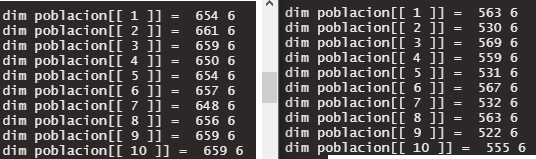
\includegraphics[width=\textwidth]{num_genes_generaciones_1_2} %scale = 0.7
%\caption[\textit{Número de genes en generaciones 1 y 2}]{\textit{Número de genes en generaciones 1 y 2}}
%\end{figure}



Sabemos que la asignación final es el mejor elemento de la última generación. En la \tablename{~\ref{submatAsigFinal}} presentamos una submatriz de la asignación final. Cabe aclarar que los datos se ordenaron con respecto a la materia (en orden alfabético) y por hora (de menor a mayor). La matriz completa se puede ver el el Apéndice \ref{Ej_AsigFinal}. Dicha matriz tiene 630 grupos asignados, cada uno con materia, profesor y horario correspondiente. En el semestre 2020-1 se tuvieron 747 grupos reales. Se simularon 1011 grupos en \textit{mat\_esqueleto}. Las materias optativas y obligatorias de los siguientes porcentajes se consideran con respecto a la carrera de Actuaría.

\begin{eqnarray*}
\dfrac{630}{1011} &=& 62.31\% \text{grupos asignados}\\
\dfrac{229}{1011} &=& 22.65\% \text{grupos de optativas sin asignación}\\
\dfrac{17}{1011} &=& 1.68\% \text{grupos de inglés sin asignación}\\
\dfrac{1011 - (630 + 229 + 17)}{1011} &=& \dfrac{135}{1011} = 13.35\% \text{grupos de obligatorias sin asignación}\\
\dfrac{630}{747} &=& 84.33\% \text{grupos asignados comparado con el 2020-1}
\end{eqnarray*}

\begin{figure}[H]
\centering
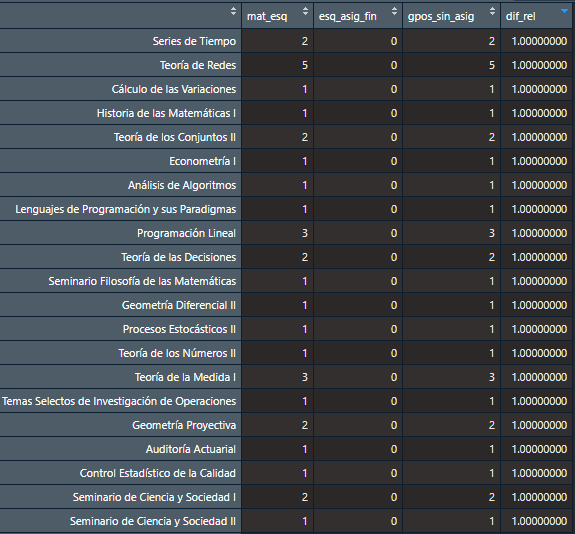
\includegraphics[width=\textwidth]{dif_rel_optativas_sin_gpo} %scale = 0.7
\caption[\textit{Optativas sin grupos asignados}]{\textit{Optativas sin grupos asignados}}
\end{figure}


\begin{table}[H]
\centering
\begin{tabular}{|c|p{7cm}|p{4.7cm}|c|}
\hline
\textbf{ } & \textbf{Materia} & \textbf{Profesor} & \textbf{Horario} \\ \hline
1 & Administración Actuarial del Riesgo & Eduardo Bello Castañeda & 7 \\ \hline
  129 & Cálculo Diferencial e Integral I & Javier Fernández García & 11 \\ \hline
  137 & Cálculo Diferencial e Integral II & Elena de Oteyza de Oteyza & 7 \\ \hline
  156 & Cálculo Diferencial e Integral III & Javier Páez Cárdenas & 11 \\ \hline
  167 & Cálculo Diferencial e Integral IV & Héctor Méndez Lango & 10 \\ \hline
  277 & Geometría Analítica I & Oscar Alfredo Palmas Velasco & 10 \\ \hline
  326 & Inferencia Estadística & Hugo Villaseñor Hernández & 19 \\ \hline
  445 & Métodos Cuantitativos en Finanzas & Irma Rocío Zavala Sierra & 8 \\ \hline
  455 & Modelos de Supervivencia y de Series de Tiempo & David Chaffrey Moreno Fernández & 8 \\ \hline
  465 & Modelos no Paramétricos y de Regresión & Margarita Elvira Chávez Cano & 10 \\ \hline
  466 & Modelos no Paramétricos y de Regresión & Jaime Vázquez Alamilla & 12 \\ \hline
  467 & Modelos no Paramétricos y de Regresión & Lizbeth Naranjo Albarrán & 13 \\ \hline
  486 & Probabilidad I & Jaime Vázquez Alamilla & 8 \\ \hline
  499 & Probabilidad II & David Josafat Santana Cobian & 10 \\ \hline
  519 & Procesos Estocásticos II & María Asunción Begoña Fernández Fernández & 10 \\ \hline
  533 & Programación & José Alfredo Cobián Campos & 15 \\ \hline
  600 & Teoría del Riesgo & Karen Lanzguerrero Obeid & 8 \\ \hline
  630 & Variable Compleja I & Jorge Hernández Hernández & 19 \\ \hline
\end{tabular}
\caption[\textit{Submatriz con asignación final}]{\textit{Se muestra una submatriz de la asignación final. Cada renglón tiene la información de un grupo con una materia, profesor y horario asignado.}}\label{submatAsigFinal}
\end{table}




